\section{Model 1: Plane Mechanics Model}

\subsection{The center of percussion}

In this part, we think that the center of percussion is the point on an object where a perpendicular impact will produce translational and rotational forces which perfectly cancel each other out at some given pivot point, so that the pivot will not be moving momentarily after the impulse. In addition, we study the reference of the Harvard University \cite{Percussion} seriously to find that we can obtain that the sweet spot is not at the end of the bat through proving the center of percussion is not in the top of bat. In the following article we will prove the center of percussion is not at the end of the bat.

Because the application time that the baseball acts on the bat is momentary, for the purpose of simplifying our model, we use the instantaneous impluse to solve the following problem. The moment when the ball hits the bat, its horizontal speed is far greater than the speed of the vertical direction, as a result, we could neglect its vertical speed in our model.

\begin{figure}[!htb]
\centering
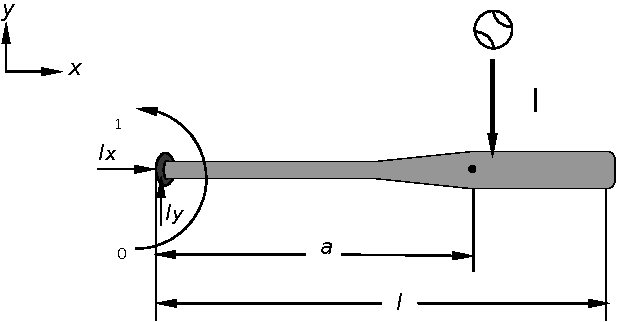
\includegraphics[width=0.6\textwidth]{batball.pdf}
\caption{\label{CollisionOfBaseballAndBat}collision of baseball and bat}
\end{figure}

By means of doing force analysis to the bat, the equations about the horizontal direction by the theorem of momentum and the momentum theorem of the vertical direction are

\begin{equation}
I_y-I=ma\omega_0-ma\omega_1, I_x=0
\end{equation}

Where
$I_y$ is the impulse that the bat to the athlete's hands in the horizontal direction,
  $I$ is the impulse that the ball to the bat,
  $a$ is the distance between the hand grip and the center of mass,
  $\omega_0$ is the bat's instantaneous angular velocity before collision,
  $\omega_1$ is the bat's instantaneous angular velocity after collision,
  $I_x$ is the impulse that the bat to the athlete's hands in the vertical direction.

In rapid sequence, we do the force analysis to the spot of the bat hand grip, and via the theorem of moment of momentum to obtain the following equation

\begin{equation}
-Ih=J\omega_0-J\omega_1
\end{equation}

Where $h$ is the distance between the hand grip and the center of percussion,
   $J$ is the moment of inertia of the bat.

As we all know that the center of percussion is the spot where the athlete's feelings are more comfortable, which means the athletes' hands are born the smallest impulse from the baseball bat, so that we can get the equation as followed

\begin{equation}
I_y=0
\end{equation}

Therefore, combine the equation 1,2,3, we have the 4th equation that is

\begin{equation}
h=\frac{J}{ma}
\end{equation}

In the following article, we will prove that $h$  is less than $l$ , meanwhile, according to the definition of moment of inertia, we can simply get the moment of inertia of the bat which is

\begin{equation}
J=\int_0^lx^2s(x)\rho\textrm{d}x
\end{equation}

Putting the above equation into the equation (4), we obtain

\[
\frac{h}{l}=\frac{\int_0^lx^2s(x)\rho\textrm{d}x}{\int_0^llxs(x)\rho\textrm{d}x}<1
\]


\textbf{Results Analysis}

By establishing and solving the above model ,we can obtain a result that $h<l$, which proves that the center of percussion is not at the end of the baseball bat, which is to say the sweet spot is not at the end of the bat. By analysising the results seriously, we find that the results match the general assumptions in our model, and what's more the results also match our expectations. Namely, it is worth pointing out are the facts that this method is in the ideal conditions (without making the errors by the player) to be raised. But in the actual baseball game, we have to take many factors into consideration, such as the weather, the competition area, the paychological factor of the athletes and so on. Besides, this method also makes the process of the hitting between the bat and the baseball ideal. This may be existent some difference when compared with the practical situation. However, as a consequence of these simplified in the real world are allowed, so we get the results of which also has a high credibility.


\subsection{The point which produces maximum batted ball speed}

Supposing the ball is being hit with the bat by direct impact, so we can know the baseball and the bat are always in the same plane of movement, Figure \ref{Motion} is a bat's trajectory\cite{EvaluatePredict}.

\begin{figure}[!htb]
\centering
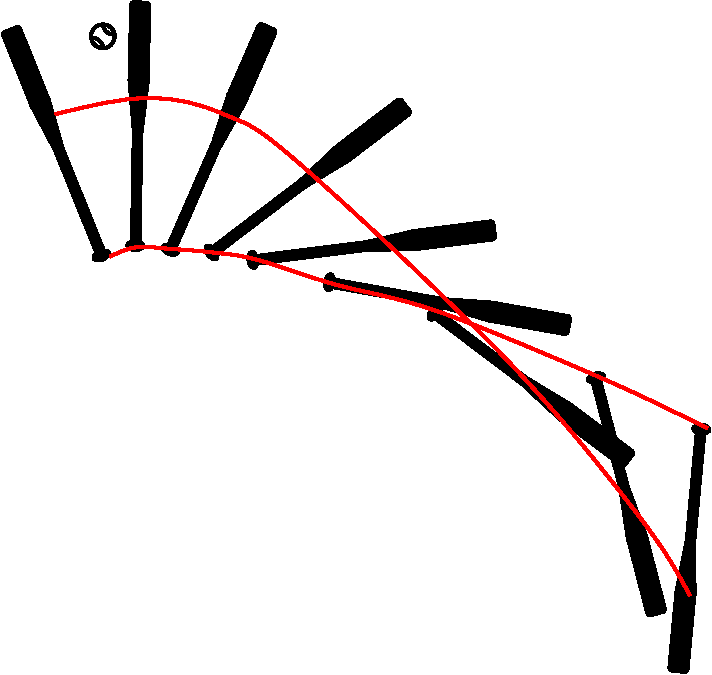
\includegraphics[width=0.6\textwidth]{motion.pdf}
\caption{\label{Motion}Motion of the swinging bat}
\end{figure}

Watts and Bahill also show that this rotational kinetic energy can be further broken down into a combination of two rotational motions, which can be used to derive an equation for batted-ball velocity. By analyzing the movement of the bat in figure \ref{Motion}, we can put its process of the motion broadly divided into two aspects of translational and rotational, as the Figure \ref{Varibales} shows. Ultimately, the process of these motions can be used to locate the bat to provide maximum energy transfer point, in other words, that is the sweet spot which the baseball can obtain the greatest speed.

\begin{figure}[!htb]
\centering
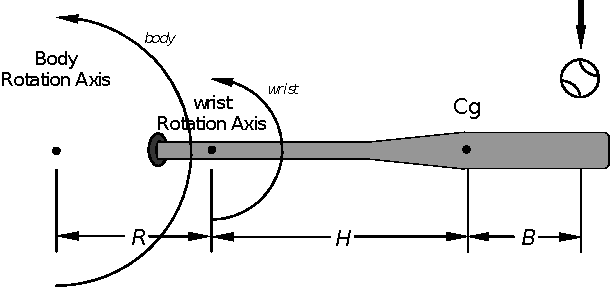
\includegraphics[width=0.6\textwidth]{basebat.pdf}
\caption{\label{Varibales}Variables denoted in swing equations}
\end{figure}


On the assumption that a batter's swing can be drawn as shown in Figure 3 where two angular velocity are applied to the bat: $\omega_{body}$ due to the rotation of the body and $\omega_{wrist}$ due to the rotation of the batter's wrists during the swing. The linear velocity of the bat at the $c_g (v_{2b})$ and at the point of impact ($v_B$) before a collision with the ball are

\[
v_{2b}=(R+H)\omega_{body}+H\omega_{wrist}
\]

\[
v_B=(R+H+B)\omega_{body}+(H+B)\omega_{wrist}
\]

Combining these two equations yields

\[
v_B=B(\omega_{body}+\omega_{wrist})+v_{2b}
\]

Making the substitution of $\omega_2 = \omega_{body} + \omega_{wrist}$ simplifies the equation further. And it is well known to us all that the total momentum for the bat and ball before and after the collision is conserved:

\begin{equation}
m_1v_{1b}+m_2(v_{2b}+\omega_{2b}B)=m_1v_{1a}+m_2(v_{2a}+\omega_{2a}B)
\end{equation}

Where $m_1$ is the mass of the ball, $m_2$ is the mass of the bat, $v_{1b}$ and $v_{1a}$ are the speed of the ball before and after collision, and $v_{b2}$ and $v_{a2}$ is the speed of the bat before and after collision.


During the bat-ball collision, we could suppose that the force exerted on the bat from the impact with the ball is $-F_1$, resulting in a torque on the bat about its $Cg$ is equal to $-BF_1$. Equating this torque over time $t$ to the change in angular momentum yields for the bat

\[
-BF_1t=I_0(\omega_{2a}-\omega_{2b})
\]

Similarly for the ball

\[
BF_1t=Bm_1(v_{1a}-v_{1b})
\]

Assuming that the rotational kinetic energy of the ball is negligible when compared to the translational kinetic energy. Conserving angular momentum between the bat and the ball during the collision produces

\begin{equation}
I_0(\omega_{2a}-\omega_{2b})+Bm_1(v_{1a}-v_{1b})=0
\end{equation}

The coefficient of restitution (COR) is defined as

\begin{equation}
e=\frac{v_{separate}}{v_{encounter}}=\frac{v_{1a}-v_{2a}-B\omega_{2a}}{v_{1b}-v_{2b}-B\omega_{2b}}
\end{equation}

where the COR is the negative ratio of the relative velocities of two bodies after and before a collision. The COR is not a value that is regarded as a material property because it not only depends on the material of both impacted bodies, but for nonlinear material systems, it also depends on the velocity at which they collide. It will also vary with respect to 9 different sizes, shapes and the temperature of the impacting bodies. For values of $e=1$, the collision is considered to be a perfectly elastic impact, that is, there is no energy loss due to the deformation of the bodies at impact. For values of $e=0$, the collision is considered to be a perfectly plastic impact. The relative velocity of the two bodies after impact is zero and the two particles move together at the same speed.

By integrating the above equations and using the Matlab software to solve, we get the baseball is shot out of a maximum speed of $v_{1a}$ (please see the annex to the \textbf{BatBallCollision.m} to get the process of the solution in detail).

\textbf{Results Analysis}


Through the solution process of the maximum speed $v_{1a}$ , we can get the result that the position of the sweet spot is not at the end of the bat. This result shows that our original conclusion concerning the position of the sweet spot is not at the end of the bat is quite correct, and it also proves that the empirical finding is wrong.

\subsection{The effect of the sweet spot of the corked bat}

The following arguments extracted from a reading of Robert Adair's book \textit{The Physics of Baseball}\cite{SwingWeights}

\begin{itemize}
\item \textbf{A corked bat has (slightly) less mass.} Because wood has been removed from the bat and replaced by some substances with a smaller density than wood, the bat is lighter by 1 to 2oz, depending on the dimensions of the cavity and the density of the filling substances. A bat which has less mass, and especially when it has a lower moment of inertia, may be swung faster. Potentially, 1.5oz does not much for an amateur player, but for a professional it means being able to watch the ball travel an additional 5 to 6 feet before having to commit to a swing.

\item \textbf{A corked bat's center of gravity closer to the hands.}Not only is the bat lighter, but the center of gravity and the balance point of the bat move closer to the hands. This means that the ''swing weight" of the bat is also reduced.

\item \textbf{A corked bat has lower inertia.} The moment of inertia (MOI) of the bat about the knob is reduced for a corked bat. You can think of the MOI as the ``rotational inertia" of the bat. Just like the ``inertia" or mass of an object measures the resistance of the object to a change in its translational motion, the rotational inertia measures the resistance to a change in its rotational motion. The effect is easy to understand: it is much easier to swing something when the weight is concentrated closer to your hands (smaller MOI) than when it is concentrated far from your hands (larger MOI).

\item \textbf{A corked bat means a less effective collision.} For a given bat speed, a heavier bat will produce a higher hit ball speed than a lighter bat. That is why the head of a golf driver is heavier than that of an iron: you want to drive the ball further. By reducing the weight at the barrel end of the bat, the efficiency of the bat is reduced, giving rise to a reduced hit ball speed and less distance on a long fly ball. This is the downside of using a corked bat.

\item \textbf{A corked bat has lower ball-bat COR (BBCOR).} Figure \ref{COR} shows a typical result for one of the bats. The plot indicates that the BBCOR is lowest for the drilled (hollow) bat. The BBCOR value for the corked bat is slightly lower than the original bat, though given the error in the measurements the results are basically indistinguishable. This result confirms the previous experiment by Alan Nathan that a corked bat does not have a trampoline effect.

\item \textbf{A corked bat could help the players make better ball control.} Because the bat is lighter and can be swung faster, a player can wait a few milliseconds longer before committing to a swing. This means he can watch the pitched ball travel about 5 to 6 or more feet before deciding to swing. For a junior player this may help make contact with the ball more often. But in other words, a corked bat will not make the ball go faster or further. Though we do not take into consideration this aspect in the Plane Mechanics model immediately, we will consider it in our following computer model.

\end{itemize}

\begin{figure}[!htb]
\centering
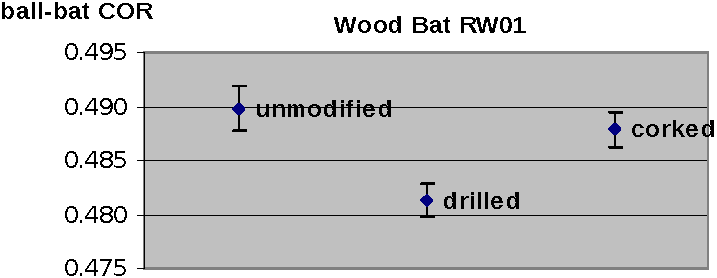
\includegraphics[width=0.8\textwidth]{batcor.pdf}
\caption{\label{COR}Measured values of the ball-bat coefficient of restitution (COR) for an unmodified, drilled, and corked wood bat, as explained in the text. The error flags indicate the standard deviation of the mean of the measurements. These data demonstrate that there is no measureable trampoline effect when a wood bat is drilled or corked.\cite{RemarksCorked}}
\end{figure}

According to the above description of the data for a corked bat, and making reference to a number of unmodified baseball bat data, we can make reasonable assumptions about the two kinds of the bat in the following analysis, as shown in the table \ref{parametersCorked}.

\begin{table}[!htb]
\centering
\caption{\label{parametersCorked}The parameters of Unmodified and Corked That we assumed}
\begin{tabular}{|l|l|l|l|l|l|}
\hline
\multicolumn{1}{|c|}{Baseball } & \multicolumn{1}{c|}{Length} & \multicolumn{1}{c|}{Weight} & \multicolumn{1}{c|}{Bp} & \multicolumn{1}{c|}{MoI6} & \multicolumn{1}{c|}{e} \\
\multicolumn{1}{|c|}{Bat} & \multicolumn{1}{c|}{($in$)} & \multicolumn{1}{c|}{($oz$)} & \multicolumn{1}{c|}{($in$)} & \multicolumn{1}{c|}{($oz-in^2$)} & \multicolumn{1}{c|}{} \\
\hline
\multicolumn{1}{|c|}{Unmodified} & \multicolumn{1}{c|}{34} & \multicolumn{1}{c|}{35} & \multicolumn{1}{c|}{22} & \multicolumn{1}{c|}{11000} & \multicolumn{1}{c|}{0.490} \\
\hline
\multicolumn{1}{|c|}{Corked} & \multicolumn{1}{c|}{34} & \multicolumn{1}{c|}{33} & \multicolumn{1}{c|}{20} & \multicolumn{1}{c|}{8000} & \multicolumn{1}{c|}{0.482} \\
\hline
\end{tabular}
\end{table}

Taking the data of table \ref{parametersCorked} into the MatLab program to get the relationship between the speed of the ball and the distance which is from the hit point to the end of the bat, and it will be shown in the figure \ref{VelocityDistance}.

\begin{figure}[!htb]
\centering
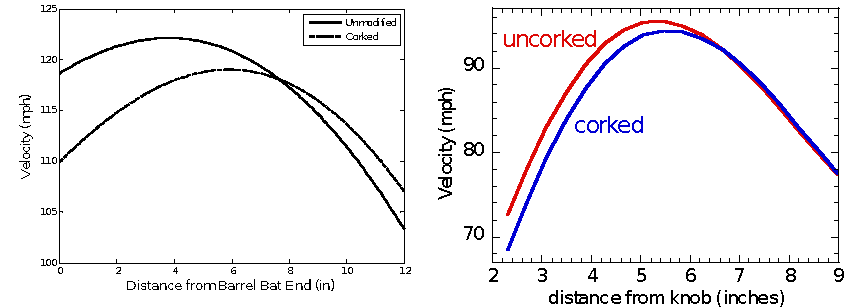
\includegraphics[width=1\textwidth]{distance.pdf}
\caption{\label{VelocityDistance}Velocity vs. Distance between collision point and Barrel Bat end.  The left figure which is we create in the model to obtain, and the right figure is extracted from the reference \cite{RemarksCorked}. By observing the analysis, we find that the results obtained in our model is are very similar with the literature. Therefore, the fact shows that to some extent our model is reasonable.}
\end{figure}


\textbf{Results Analysis}

We can see that in the the figure 5, both the results in the literature and the results of our paper could be seen that a corked bat will not play longer than the uncorked bat. By this model, we can deny that the cocked bat performs better than the traditional bat.

\begin{itemize}
\item The maximal velocity of the uncorked bat is slight bigger than the cocked bat.

\item The sweet spot of the uncorked bat is more close to the end of the bat than the corked bat.

\item The sweet spot zone of the uncorked bat is wider than the corked bat.
\end{itemize}

We conclude that the main reason may be that we do not consider the ball control factor, and we also think the reference did also not take the factor into consideration. However, we will take it into account in the following computer model, and make a further explanation that the effect which the corked bat makes.

\subsection{The differences between the wood and aluminum bats }

It is known to all that the physical differences between wood and metal baseball bats are quite obvious. But if both of them have the same mass, their structure will be very different, the metal bat must be hollow. In this part, we think the effect of the aluminum is better than the wood bat when use them to hit the baseball.

Usually, a solid wood bat weighs 2 units less than its length, on the other hand, a hollow metal bat weighs either 3 or more units less than its length. In addition to the above different factors between wood and metal baseball bats, a significant difference between wood and metal bats is the energy-transfer mechanism between the bat and the baseball during the collision.

However, the difference between the energy-transfer mechanisms is a fundamental result of the wood bat being solid and the metal bat being hollow.That is to say that we can create a model to predict the different behavior about wood(usually ash) or metal(usually aluminum) bats.

In our model, we also use the wood and aluminum bat to solve the problem. There is some information with regard to the two different types of the bats as shown in the table and figure \ref{correspondingparameters}\cite{hollowsoftball}.

\begin{figure}[!htb]
\centering
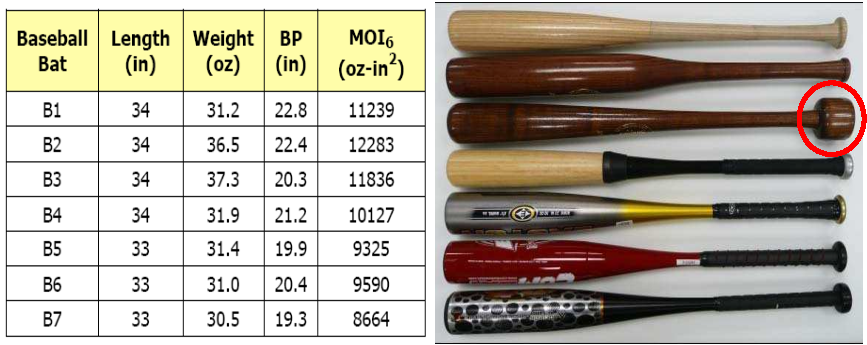
\includegraphics[width=0.8\textwidth]{figtab.pdf}
\caption{\label{correspondingparameters}Different bats and their corresponding parameters\cite{Swing_Weights}}
\end{figure}


We can demonstrably know the weight, balance point and moment of inertia about 6-in point on the hand grip on the bat by a sampling of 34-inch wood baseball and 33-inch aluminum or composite bats comparing combinations in the figure \ref{correspondingparameters}(left). Simultaneously, we give a figure whose different bats via descending order from top to bottom are one-to-one correspondence with the parameters in the figure \ref{correspondingparameters}(left). Quite obviously, we find that the third bat is different from the other bats in the figure \ref{correspondingparameters}(right), and we have already come out it with a red circle. We caculate this will make some different results in our following plot. \cite{hollowsoftball}

In addition, there are extra difference that we must take into account.

\begin{itemize}
\item \textbf{Aluminum bats can be swung faster.} Comparison of wood and aluminum bats, an aluminum bat with the same weight as a wood bat will have a significantly lower inertia and a player can swing a lower inertia bat faster.(we set aluminum bat velocity = 106.5 and wood = 98.6)

\item Aluminum bats have the ``trampoline effect". When a ball hits a wood bat, it compresses to nearly half its original diameter, losing up to 75\% of its initial energy to internal friction forces during this compression. In a hollow bat, however, the bat barrel compresses somewhat like a spring, when the ball impacts it.(we set aluminum bat COR = 0.5 and wood =0.45);
\end{itemize}

By substituting the different parameters of the baseball bats in the figure 6(left)into the $v_{1b}=F(B,L,m,BP,I)$ representative values for wood and metal bats, a plot of the batted-ball velocity as a function of the location of the impact point on the bat from the barrel end can be created.


\begin{figure}[!htb]
\centering
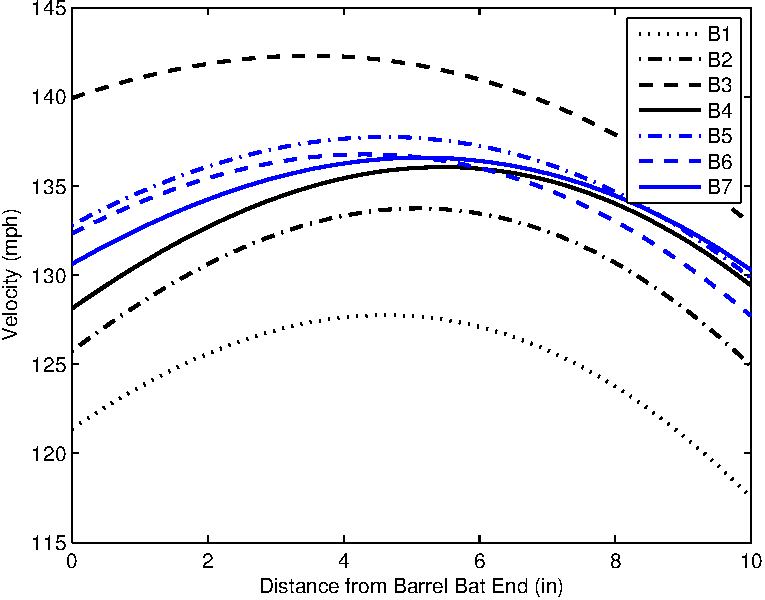
\includegraphics[width=0.6\textwidth]{fig01m1.pdf}
\caption{\label{Plotdemonstrating}Plot demonstrating Equation}
\end{figure}

In this figure, combining the maximum speed $v_{1b}=F(B,L,m,BP,I)$ we can obtain the functional relations between the maximum speed and the distance from striking point on the ball to the end of the bat. We can easily find that the place where the sweet spot on the bat is and the B3 curve is different from the other curves distinctly. Namely, we also find the metal bat is better than the wood bat when used to hit the baseball in the figure.

\textbf{Results Analysis}

From the above figure \ref{Plotdemonstrating}, we can come to the results that:

\begin{itemize}

\item \textbf{The peaks show where along the length of the bat the maximum energy transfer occurs.} We obtain the result the location of the maximum energy transfer is commonly referred to as the sweet spot on the bat, at the same time it proves the sweet spot is not at the end of the bat again and explains our previous model is correct and feasible again.

\item \textbf{Both the materials and the shape structure will have an effect on the ``sweet spot" effect.}
 We find that the B3 curve is different from the others, this responds our previous conclusion that its special structure makes it different, on the other hand, this explains that our model is feasible.

\item \textbf{The aluminum bat is better than the wood bat.} We analyze the differences between the wood and metal bat with the figure \ref{Plotdemonstrating}, and we get the result that the aluminum bat is better than the wood bat. This also explains the different materials have effects on batting. But on account of the aluminum bat can hit the baseball faster and farther, it makes the athletic competition reduce more, and it is also unfair to the competitors who use the wood bat. Therefore, for the purpose of the principle of athletic and fair play, the metal wood should be prohibited in the baseball game. Maybe it is the reason why Major League Baseball prohibits metal bats. However, for a beginner the metal bat is still a better tool to learn.

\end{itemize}
